\title{\textsc{CORN}}
\author{Giorgio Giuffr\`e \\ 1069456}
\date{}

\documentclass[12pt]{article}
\usepackage[utf8]{inputenc}
\usepackage{mathtools}
\usepackage{amssymb}
\usepackage{tikz}
\usepackage{tkz-graph}
\renewcommand*{\EdgeLineWidth}{0.15pt}

\tikzset{
	every neuron/.style={
		circle,
		draw,
		minimum size=1cm
	},
	neuron missing/.style={
		draw=none, 
		scale=4,
		text height=0.333cm,
		execute at begin node=\color{black}$\vdots$
	},
}



\begin{document}
\maketitle



%%% ========================================
%%% ========================================

\begin{abstract}
\textsc{CORN} (COstruttore di Reti Neurali) è una piccola piattaforma che permette di progettare e allenare semplici reti neurali artificiali, per poi  testarle su input numerici.
\end{abstract}



%%% ========================================
%%% ========================================

\section{Introduzione}

\subsection{Cos'è una rete neurale?}

\paragraph{}
Il miglior esempio di rete neurale è senz'altro il cervello umano: una rete di cellule collegate tra loro, dette neuroni, alcune delle quali si interfacciano con l'ambiente esterno (i neuroni sensoriali e i neuroni motori) mentre altre stanno “nascoste” dall'esterno, nei meandri della rete. Ciò che succede nel cervello umano è abbastanza caotico: ogni neurone manda segnali a più neuroni e riceve segnali da neuroni diversi, determinando un'intricata catena parallela di segnali che termina con i neuroni motori, collegati ai muscoli delle gambe, della bocca, delle mani eccetera.

\paragraph{}
In poche parole, una rete neurale è un grafo orientato in cui ogni nodo è un \textbf{neurone} e ogni arco è un \textbf{segnale} che viene mandato da un neurone a un altro. Un neurone è una cellula che riceve uno o più segnali di input, li somma ed emette un solo segnale di output (quindi è una funzione $f : \mathbb{R}^n \rightarrow \mathbb{R}$, dove $n \ge 1$ è il numero di segnali in ingresso). In base al segnale totale di input $x$, ogni neurone emette quindi un certo segnale di output $f(x)$ che può poi ramificarsi, cioè può essere mandato a più di un neurone, a seconda di com'è disegnato il grafo. Le connessioni (gli archi) tra un neurone e l'altro sono pesate, cioè ogni input $x_i$ viene moltiplicato per una costante reale $w_i$ che può essere modificata dalla rete nel corso del tempo.

\paragraph{}
Tutti i neuroni della rete implementano la stessa semplice funzione $f$, detta \textbf{funzione di attivazione}. Chiaramente, l'output di due neuroni può essere diverso, per il fatto che gli archi della rete non hanno tutti lo stesso peso. La capacità di modificare i pesi delle proprie connessioni fa sì che la rete sia capace di associare ad ogni input un certo output desiderato. Ad esempio, una rete con due neuroni di input e un neurone di output (oltre ad eventuali neuroni intermedi), può modificare i propri pesi in modo da imparare a calcolare la media di due numeri che le vengono presentati:

\begin{center}
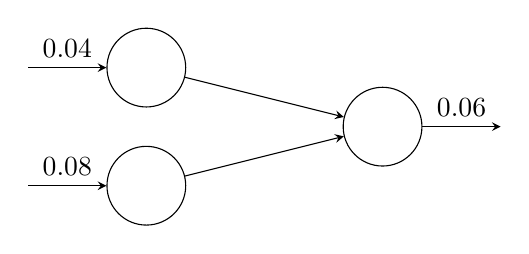
\begin{tikzpicture}[x=1.5cm, y=1.5cm, >=stealth]

\foreach \m/\l [count=\y] in {1,2}
	\node [every neuron/.try, neuron \m/.try] (input-\m) at (0,2-\y) {};

\foreach \m [count=\y] in {1}
	\node [every neuron/.try, neuron \m/.try ] (output-\m) at (2,1.5-\y) {};

\foreach \l [count=\i] in {0.04, 0.08}
	\draw [<-] (input-\i) -- ++(-1,0)
		node [above, midway] {$\l$};

\foreach \l [count=\i] in {0.06}
	\draw [->] (output-\i) -- ++(1,0)
		node [above, midway] {$\l$};

\foreach \i in {1,2}
	\foreach \j in {1}
		\draw [->] (input-\i) -- (output-\j);

\end{tikzpicture}
\end{center}

La rete apprende grazie ad una serie di \textbf{esempi} che le vengono presentati: $(0.04, 0.08 \rightarrow 0.06)$, $(0.05, 0.01 \rightarrow 0.03)$, $(0.02, 0.05 \rightarrow 0.035)$, $(0.09, 0.08 \rightarrow 0.085)$ e così via. Più esempi vengono forniti, più è preciso l'apprendimento.

\paragraph{}
Oppure, una rete con 4 neuroni in ingresso e 4 in uscita potrebbe imparare a calcolare il successore di un numero in formato binario:

\begin{center}
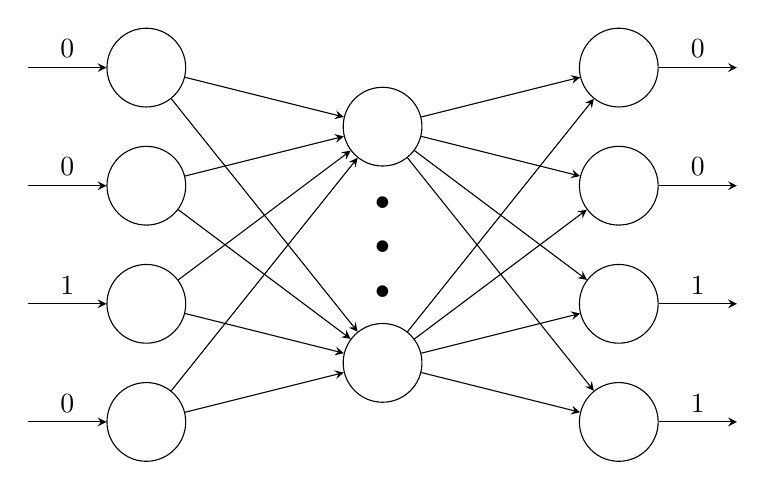
\begin{tikzpicture}[x=1.5cm, y=1.5cm, >=stealth]

\foreach \m/\l [count=\y] in {1,2,3,4}
	\node [every neuron/.try, neuron \m/.try] (input-\m) at (0,2-\y) {};

\foreach \m/\l [count=\y] in {1,missing,2}
	\node [every neuron/.try, neuron \m/.try] (hidden-\m) at (2,1.5-\y) {};

\foreach \m [count=\y] in {1,2,3,4}
	\node [every neuron/.try, neuron \m/.try ] (output-\m) at (4,2-\y) {};

\foreach \l [count=\i] in {0, 0, 1, 0}
	\draw [<-] (input-\i) -- ++(-1,0)
		node [above, midway] {$\l$};

\foreach \l [count=\i] in {0, 0, 1, 1}
	\draw [->] (output-\i) -- ++(1,0)
		node [above, midway] {$\l$};

\foreach \i in {1,...,4}
	\foreach \j in {1,...,2}
		\draw [->] (input-\i) -- (hidden-\j);

\foreach \i in {1,...,2}
	\foreach \j in {1,...,4}
		\draw [->] (hidden-\i) -- (output-\j);

\end{tikzpicture}
\end{center}

\subsection{Cosa può fare \textsc{CORN}?}

\paragraph{}
Insomma, i compiti che una rete può imparare sono numerosissimi e \textsc{CORN} si propone di offrire un'interfaccia semplice per specificare sia la configurazione della rete sia i compiti da farle imparare. La creazione di una rete neurale artificiale si articola in tre fasi: Definizione dell'architettura della rete; definizione di alcuni esempi da presentare alla rete; allenamento della rete.



%%% ========================================
%%% ========================================

\section{Guida all'uso}

...



%%% ========================================
%%% ========================================

\section{Implementazione}

\subsection{Parte logica}

\begin{center}
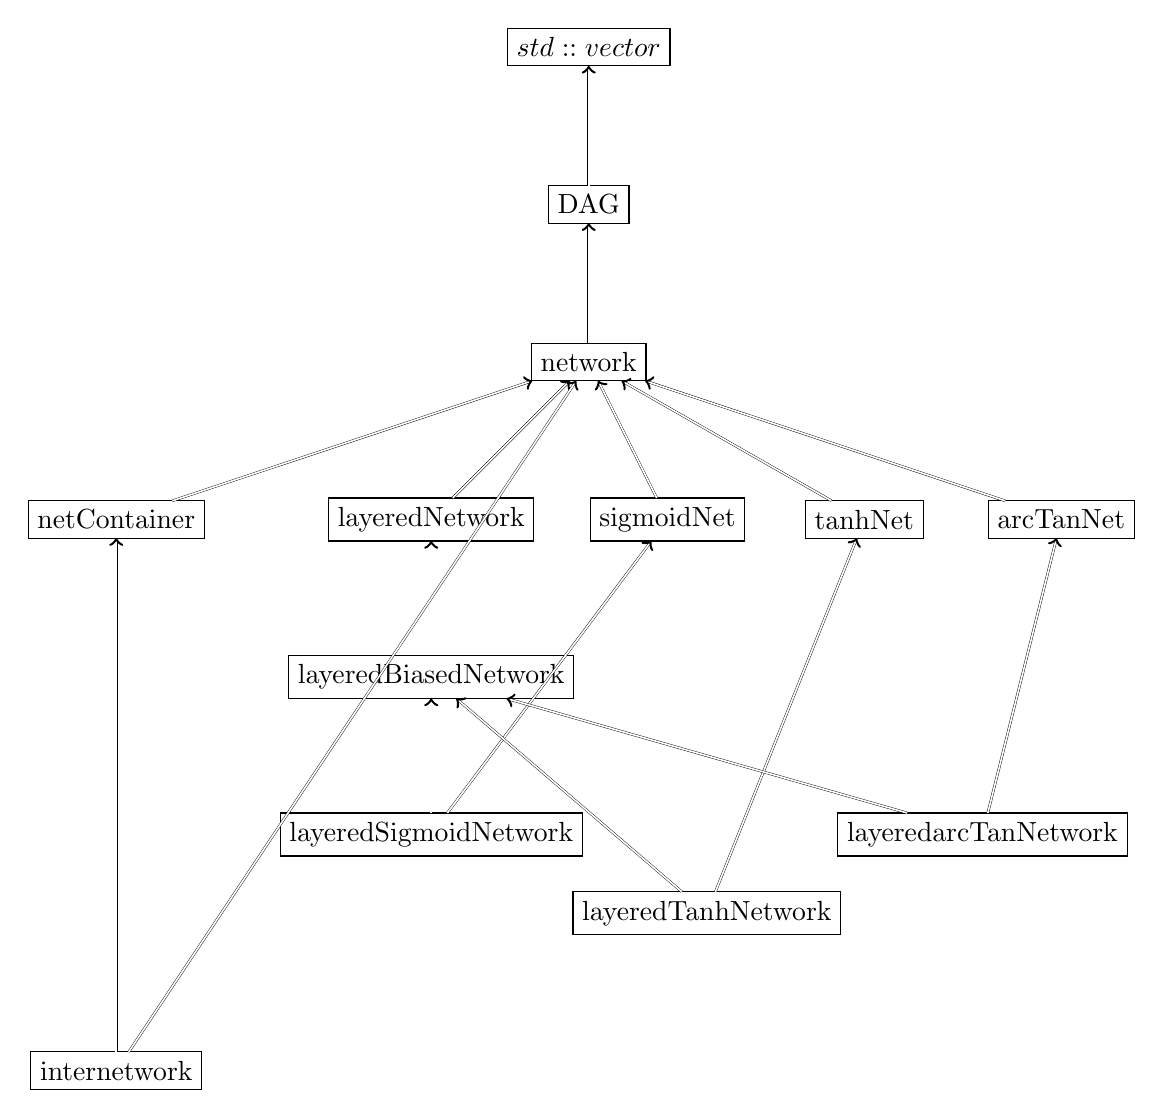
\begin{tikzpicture}
%\SetVertexNormal[Shape = rectangle,
%				Fill = white]
\tikzset{VertexStyle/.style = {
		shape = rectangle,
		fill = white,
		draw}}
\tikzset{EdgeStyle/.style = {
		->,
		double distance = 0.6pt}}

\Vertex[L=$std::vector$] {vector}
	\Vertex[x=0,y=-2]{DAG}
		\Vertex[x=0,y=-4]{network}
			\Vertex[x=-6,y=-6]{netContainer}
			\Vertex[x=-2,y=-6]{layeredNetwork}
				\Vertex[x=-2,y=-8]{layeredBiasedNetwork}
			\Vertex[x=1,y=-6]{sigmoidNet}
			\Vertex[x=3.5,y=-6]{tanhNet}
			\Vertex[x=6,y=-6]{arcTanNet}

					\Vertex[x=-2,y=-10]{layeredSigmoidNetwork}
					\Vertex[x=1.5,y=-11]{layeredTanhNetwork}
					\Vertex[x=5,y=-10]{layeredarcTanNetwork}

					\Vertex[x=-6,y=-13]{internetwork}

\Edges(DAG,vector)
\Edges(network,DAG)
\Edges(layeredNetwork,network)
\Edges(netContainer,network)
\Edges(layeredBiasedNetwork,layeredNetwork)
\Edges(sigmoidNet,network)
\Edges(tanhNet,network)
\Edges(arcTanNet,network)
\Edges(layeredSigmoidNetwork,sigmoidNet)
\Edges(layeredSigmoidNetwork,layeredBiasedNetwork)
\Edges(layeredTanhNetwork,tanhNet)
\Edges(layeredTanhNetwork,layeredBiasedNetwork)
\Edges(layeredarcTanNetwork,arcTanNet)
\Edges(layeredarcTanNetwork,layeredBiasedNetwork)
\Edges(internetwork,network)
\Edges(internetwork,netContainer)

\end{tikzpicture}
\end{center}

\subsection{Interfaccia grafica}

...



\end{document}
